%!TEX root = ../main.tex

\chapter{CNN Vowel Recognition Model}
\label{chp:model}

\paragraph{}
This chapter presents a detailed description of our CNN-based vowel recognition system, encompassing the complete pipeline from data preparation to model evaluation. We begin by examining the audio data preparation process, which includes the generation and processing of vowel sounds using multiple text-to-speech synthesis libraries. The chapter then explores the conversion of audio data into spectrograms, which serve as the visual input for our CNN model. This transformation process is crucial as it allows us to leverage the powerful pattern recognition capabilities of CNNs in the visual domain for audio classification tasks. Finally, we present our testing methodology and results, demonstrating the model's effectiveness in real-world applications. Throughout the chapter, we emphasize the technical decisions and optimizations that contribute to the system's robust performance in vowel recognition tasks.

\paragraph{}
Recent advances in deep learning approaches \cite{deep_speech2023} have shown significant improvements in speech recognition accuracy. Our implementation builds upon these developments, incorporating modern acoustic analysis methods \cite{acoustic_analysis2023} and advanced formant analysis techniques \cite{formant_analysis2022}.

\section{Audio Data Preparation}
The project includes a robust audio generation pipeline for creating training data using three different text-to-speech synthesis libraries for maximum versatility and quality.

\subsection{Voice Synthesis Libraries}

\subsubsection{Pyttsx3 Library}
\paragraph{}
The first implementation utilizes Pyttsx3, which leverages local system voices. This approach prioritizes finding and utilizing Italian voices for authentic vowel pronunciation, with a fallback mechanism to default system voices when Italian voices are unavailable.

\begin{lstlisting}[language=Python, caption={Audio Generation with pyttsx3}]

    import os
    import numpy as np
    from scipy.signal import lfilter
    from pydub import AudioSegment
    import pyttsx3
    import soundfile as sf
    from scipy.signal import butter, filtfilt
    
    def get_italian_voice():
        """
        Find an Italian voice from available system voices.
        """
        engine = pyttsx3.init()
        voices = engine.getProperty('voices')
        for voice in voices:
            if 'italian' in voice.name.lower() or 'it' in voice.id.lower():
                return voice.id
        return None
    
    def generate_vowel(vowel, duration=1000, variation=0):
        """
        Generate an Italian vowel sound using text-to-speech synthesis with significant variations.
        :param vowel: The vowel character ('A', 'E', 'I', 'O', 'U')
        :param duration: Duration in milliseconds
        :param variation: Variation index for differentiation
        :return: AudioSegment object
        """
        engine = pyttsx3.init()
        italian_voice = get_italian_voice()
        if italian_voice:
            engine.setProperty('voice', italian_voice)
        else:
            print("Warning: No Italian voice found. Using default voice.")
        
        # Expanded variations without pitch (SAPI5 compatible)
        rates = [60, 80, 100, 120, 140, 160, 180, 200, 220, 240]  # More speed variations
        volumes = [0.3, 0.4, 0.6, 0.8, 1.0, 1.2, 1.4, 1.6, 1.8]   # More volume variations
        
        # Use modulo to cycle through variations
        rate_idx = variation % len(rates)
        volume_idx = (variation // len(rates)) % len(volumes)
        
        engine.setProperty('rate', rates[rate_idx])
        engine.setProperty('volume', volumes[volume_idx])
        
        return engine, vowel
    
    def add_noise_and_filter(audio_file, noise_level=0.005, cutoff=3000):
        """
        Add noise and apply a low-pass filter to an audio file.
        """
        data, samplerate = sf.read(audio_file)
        noise = np.random.normal(0, noise_level, data.shape)
        data_noisy = data + noise
    
        nyquist = 0.5 * samplerate
        normal_cutoff = cutoff / nyquist
        b, a = butter(6, normal_cutoff, btype='low', analog=False)
        filtered_data = filtfilt(b, a, data_noisy)
        
        sf.write(audio_file, filtered_data, samplerate)
    
    def change_pitch(audio_file, semitones):
        """
        Change pitch of an audio file by a given number of semitones.
        """
        sound = AudioSegment.from_file(audio_file, format="wav")
        new_sample_rate = int(sound.frame_rate * (2.0 ** (semitones / 12.0)))
        return sound._spawn(sound.raw_data, overrides={'frame_rate': new_sample_rate}).set_frame_rate(44100)
    
    # Generate and export vowel variations
    duration = 1000  # milliseconds
    num_variations = 200  # Increased to 800 variations
    vowel_folders = ['A', 'E', 'I', 'O', 'U']
    pitch_variations = [-2, -1, 0, 1, 2]  # Semitones to shift
    
    for vowel in vowel_folders:
        os.makedirs(vowel, exist_ok=True)
        for variation in range(num_variations):
            engine, vowel_sound = generate_vowel(vowel, duration, variation)
            base_filename = f"{vowel}/{vowel}_vars{variation}.wav"
            engine.save_to_file(vowel_sound, base_filename)
            engine.runAndWait()
            
            # Add noise and filter
           # add_noise_and_filter(base_filename)
            
            # Apply pitch variations
            for semitones in pitch_variations:
                if semitones != 0:  # Skip pitch change for original pitch
                    pitched_audio = change_pitch(base_filename, semitones)
                    pitch_filename = f"{vowel}/{vowel}_varr{variation}_pitch{semitones}.wav"
                    pitched_audio.export(pitch_filename, format="wav")
            
            print(f"Generated {base_filename} with variations")


\end{lstlisting}

\subsubsection{Microsoft Edge TTS}
\paragraph{}
The second implementation employs Microsoft Edge's Text-to-Speech service through Edge-TTS. This cloud-based solution provides high-quality voice synthesis that maintains consistent quality across different systems. The service's reliability and standardized output make it particularly valuable for generating training data.

\begin{lstlisting}[language=Python, caption={Audio Generation with Edge TTS}]

    import os
    import asyncio
    import edge_tts
    import numpy as np
    import soundfile as sf
    from pydub import AudioSegment
    
    async def generate_vowel_edge(vowel, variation=0):
        """
        Generate an Italian vowel sound using Edge TTS with variations.
        :param vowel: The vowel character ('A', 'E', 'I', 'O', 'U')
        :param variation: Variation index for differentiation
        :return: Path to temporary audio file
        """
        # Only female Italian voices
        voices = [
            "it-IT-ElsaNeural",       # Female voice 1
            "it-IT-IsabellaNeural",   # Female voice 2
        ]
        
        # Variation parameters
        rates = ["-20%", "-10%", "0%", "+10%", "+20%"]
        pitches = ["-100Hz", "-50Hz", "0Hz", "+50Hz", "+100Hz"]
        volumes = ["-20%", "-10%", "0%", "+10%", "+20%"]
        
        # Use variation to cycle through parameters
        voice_idx = variation % len(voices)
        rate_idx = (variation // len(voices)) % len(rates)
        pitch_idx = (variation // (len(voices) * len(rates))) % len(pitches)
        volume_idx = (variation // (len(voices) * len(rates) * len(pitches))) % len(volumes)
        
        communicate = edge_tts.Communicate(
            vowel,
            voices[voice_idx],
            rate=rates[rate_idx],
            volume=volumes[volume_idx],
            pitch=pitches[pitch_idx]
        )
        
        # Create temporary file
        temp_file = f"temp_{vowel}_{variation}.wav"
        await communicate.save(temp_file)
        return temp_file
    
    def change_pitch(audio_file, semitones):
        """
        Change pitch of an audio file by a given number of semitones.
        :param audio_file: Path to input audio file
        :param semitones: Number of semitones to shift (+/-)
        :return: AudioSegment with adjusted pitch
        """
        # Read audio data using soundfile first
        data, samplerate = sf.read(audio_file)
        
        # Convert to mono if stereo
        if len(data.shape) > 1:
            data = data.mean(axis=1)
        
        # Save as temporary WAV file
        temp_wav = f"temp_pitch_{os.path.basename(audio_file)}"
        sf.write(temp_wav, data, samplerate, 'PCM_16')
        
        # Process with pydub
        sound = AudioSegment.from_wav(temp_wav)
        new_sample_rate = int(sound.frame_rate * (2.0 ** (semitones / 12.0)))
        pitched = sound._spawn(sound.raw_data, overrides={
            'frame_rate': new_sample_rate
        }).set_frame_rate(44100)
        
        # Clean up temporary file
        os.remove(temp_wav)
        
        return pitched
    
    async def main():
        # Generate and export vowel variations
        num_variations = 200
        vowel_folders = ['A', 'E', 'I', 'O', 'U']
        pitch_variations = [-2, -1, 0, 1, 2]  # Semitones to shift
    
        for vowel in vowel_folders:
            os.makedirs(vowel, exist_ok=True)
            for variation in range(num_variations):
                try:
                    # Generate base audio
                    temp_file = await generate_vowel_edge(vowel, variation)
                    base_filename = f"{vowel}/{vowel}_var{variation}.wav"
                    
                    # Read and write using soundfile to ensure correct WAV format
                    data, samplerate = sf.read(temp_file)
                    sf.write(base_filename, data, samplerate, 'PCM_16')
                    
                    # Apply pitch variations
                    for semitones in pitch_variations:
                        if semitones != 0:
                            pitched_audio = change_pitch(base_filename, semitones)
                            pitch_filename = f"{vowel}/{vowel}_var{variation}_pitch{semitones}.wav"
                            pitched_audio.export(pitch_filename, format="wav")
                    
                    # Clean up temporary file
                    os.remove(temp_file)
                    print(f"Generated {base_filename} with variations")
                    
                except Exception as e:
                    print(f"Error processing {vowel} variation {variation}: {str(e)}")
                    continue
    
    if __name__ == "__main__":
        # Install required packages if not already installed
        try:
            import edge_tts
        except ImportError:
            import pip
            pip.main(['install', 'edge-tts'])
            import edge_tts
    
        # Run the async main function
        asyncio.run(main())
    



\end{lstlisting}

\subsubsection{Google Text-to-Speech (gTTS)}
\paragraph{}
Google Text-to-Speech (gTTS) serves as the third implementation, offering extensive vowel variations. This implementation includes standard pronunciations, extended vowels, emphasized forms, combined forms, and soft pronunciations. The system implements careful filtering to remove incorrect pronunciations, ensuring data quality.

\begin{lstlisting}[language=Python, caption={Audio Generation with gTTS}]

    from gtts import gTTS
    import os
    import random
    import numpy as np
    
    # Output folder
    output_dir = "audio"
    os.makedirs(output_dir, exist_ok=True)
    
    # Define Italian vowels with more variations
    vowel_variations = {
        "a": [
            "Ah", "Aah", "Ahh", "Ahhh", "Aaah",
            "Aaaah", "Aaaaah", "Aaaaaah", "Aaaaaaah",
            "AH", "AAH", "AAHH", "AAHHH",
            "Aha", "Ahaa", "Aaha", "Aahaa",
            "ah", "aah", "ahh", "ahhh",
            # 变调
            "Aah?", "Ahh!", "Aaah~", "Ahhh~"
        ],
        "e": [
            "Eh", "Eeh", "Ehh", "Ehhh", "Eeeh",
            "Eeeeh", "Eeeeeh", "Eeeeeeh", "Eeeeeeeh",
            "EH", "EEH", "EEHH", "EEHHH",
            "Ehe", "Ehee", "Eehe", "Eehee",
            "eh", "eeh", "ehh", "ehhh",
            "Eeh?", "Ehh!", "Eeeh~", "Ehhh~"
        ],
        "i": [
            "Ee", "Eee", "Ii", "Iii", "Iiii",
            "Eeee", "Eeeee", "Iiii", "Iiiii",
            "EE", "EEE", "II", "III",
            "Eei", "Eeii", "Ieei", "Iiei",
            # 轻音
            "ee", "eee", "ii", "iii",
            # 变调
            "Ee?", "Ii!", "Eee~", "Iii~"
        ],
        "o": [
            "Oh", "Ooh", "Ohh", "Ohhh", "Oooh",
            "Ooooh", "Oooooh", "Ooooooh", "Oooooooh",
            "OH", "OOH", "OOHH", "OOHHH",
            "Oho", "Ohoo", "Ooho", "Oohoo",
            "oh", "ooh", "ohh", "ohhh",
            "Ooh?", "Ohh!", "Oooh~", "Ohhh~"
        ],
        "u": [
            "Oo", "Ooo", "Uu", "Uuu", "Uuuu",
            "Oooo", "Ooooo", "Uuuu", "Uuuuu",
            "OO", "OOO", "UU", "UUU",
            "Oou", "Oouu", "Uoou", "Uuou",
            "oo", "ooo", "uu", "uuu",
            "Oo?", "Uu!", "Ooo~", "Uuu~"
        ]
    }
    
    # TTS parameters for variation
    speeds = [False, True]  # False for normal speed, True for slow
    languages = ['it', 'it-IT']  # Different Italian language codes
    
    def generate_variations(text, base_name, vowel_dir, index):
        """Generate multiple variations of the same text with different parameters"""
        variations = []
        
        # Add slight random variations to the text
        texts = [
            text,
            text.replace('h', 'hh', random.randint(0, 1)),
            text.lower(),
            text.upper(),
            text + text[0].lower()
        ]
        
        for i, variation_text in enumerate(texts):
            for speed in speeds:
                for lang in languages:
                    try:
                        output_file = os.path.join(
                            vowel_dir, 
                            f"{base_name}_var_{index}_{i}_{speed}_{lang}.wav"
                        )
                        
                        # Add random pitch and rate variations
                        tts = gTTS(
                            text=variation_text,
                            lang=lang,
                            slow=speed
                        )
                        tts.save(output_file)
                        variations.append(output_file)
                        print(f"Saved: {output_file}")
                    except Exception as e:
                        print(f"Error generating {output_file}: {e}")
                        continue
        
        return variations
    
    # Generate sounds for each vowel
    for vowel, variations in vowel_variations.items():
        # Create subdirectory for each vowel
        vowel_dir = os.path.join(output_dir, vowel)
        os.makedirs(vowel_dir, exist_ok=True)
        
        print(f"\nGenerating sounds for vowel '{vowel}'...")
        
        # Generate each variation
        all_variations = []
        for idx, text in enumerate(variations, 1):
            generated = generate_variations(text, vowel, vowel_dir, idx)
            all_variations.extend(generated)
        
        print(f"Generated {len(all_variations)} variations for vowel {vowel}")
    
    print("\nAll vowel variations have been generated!")
    

\end{lstlisting}

\paragraph{}
The gTTS implementation generates huge amount of audio files, which is not practical for our purpose. However, due to technical reasons, there are some audio files generated by gTTS that are not included in the dataset for its low quality. After file selection, the dataset contains 1000 audio files for each vowel.
\subsection{Online Audio File Collection}
\paragraph{}
In addition to synthesized audio, the project incorporates audio samples from online Italian videos, both as trimmed segments and complete downloads, to enhance the training dataset's diversity. This collection process ensures a wide range of authentic vowel pronunciations, contributing to the robustness of the training data.

\paragraph{}
The combination of these methods ensures comprehensive coverage and quality in training data generation, providing a diverse dataset for the vowel recognition model.

\subsection{File Organization}
\label{subsec:file-organization}

\paragraph{}
The project implements a systematic file organization structure to manage the large volume of audio data efficiently. Audio files are organized into separate folders for each vowel (A, E, I, O, U), with consistent naming conventions for different types of files:

\begin{itemize}
    \item \textbf{Base Files:}
    \begin{itemize}
        \item Pattern: \texttt{[vowel]\_vars[variation].wav}
        \item Example: \texttt{A\_vars1.wav}
        \item Purpose: Standard vowel recordings without modifications
    \end{itemize}
    
    \item \textbf{Pitched Variations:}
    \begin{itemize}
        \item Pattern: \texttt{[vowel]\_varr[variation]\_pitch[semitones].wav}
        \item Example: \texttt{A\_varr1\_pitch2.wav}
        \item Purpose: Recordings with altered pitch for training diversity
    \end{itemize}
    
    \item \textbf{gTTS Generated Files:}
    \begin{itemize}
        \item Pattern: \texttt{[vowel]\_var\_[index]\_[variation]\_[speed]\_[lang].wav}
        \item Example: \texttt{A\_var\_1\_2\_1.0\_it.wav}
        \item Purpose: Files generated using Google Text-to-Speech
    \end{itemize}
    
    \item \textbf{External Resources:}
    \begin{itemize}
        \item Pattern: \texttt{[vowel]\_[index].wav}
        \item Example: \texttt{A\_1.wav}
        \item Purpose: Audio files from online or external sources
    \end{itemize}
\end{itemize}

\paragraph{}
This organized structure facilitates efficient data management and ensures:
\begin{itemize}
    \item Easy access and retrieval of specific audio files
    \item Clear traceability of file origins and modifications
    \item Scalable integration of new data sources
    \item Consistent naming across the entire dataset
    \item Enhanced reproducibility of experiments
\end{itemize}

\section{Spectrogram Generation}
\label{sec:spectrogram-generation}

\paragraph{}
After generating the audio data, the next crucial step in our pipeline is converting these audio samples into visual representations that can be processed by our CNN model. We developed a specialized image generation system that converts audio files into mel-spectrograms while preserving the essential acoustic features necessary for vowel recognition.

\subsection{Image Generation Pipeline}
\label{subsec:image-generation-pipeline}

\paragraph{}
The image generation process is implemented through a Python script that utilizes librosa for audio processing and matplotlib for visualization. The system processes audio files systematically, maintaining the organizational structure of the dataset by creating corresponding directories for each vowel category. The core functionality includes mel-spectrogram computation with carefully tuned parameters to capture the relevant frequency characteristics of vowel sounds.

\begin{lstlisting}[language=Python, caption={Spectrogram Generation with Formant Analysis}]
import os
import librosa
import librosa.display
import matplotlib.pyplot as plt
import numpy as np
from scipy.signal import find_peaks
import parselmouth
from parselmouth.praat import call

def create_output_dirs(output_dir, classes):
    for label in classes:
        os.makedirs(os.path.join(output_dir, label), exist_ok=True)

def extract_formants(audio_path, max_formant=5500, num_formants=5):
    sound = parselmouth.Sound(audio_path)
    formant = call(sound, "To Formant (burg)", 0.0, num_formants, 
                  max_formant, 0.025, 50)
    
    t = sound.duration / 2
    formants = []
    for i in range(1, num_formants + 1):
        try:
            formant_freq = call(formant, "Get value at time", 
                              i, t, 'Hertz', 'Linear')
            formants.append(formant_freq)
        except:
            formants.append(0)
    return formants

def save_spectrogram_with_formants(audio_path, output_dir, label, file_name):
    y, sr = librosa.load(audio_path, sr=None)
    
    formants = extract_formants(audio_path)
    
    n_fft = 2048
    hop_length = 512
    mel_spect = librosa.feature.melspectrogram(
        y=y,
        sr=sr,
        n_fft=n_fft,
        hop_length=hop_length,
        n_mels=128,
        fmin=20,
        fmax=8000
    )
    
    mel_spect_db = librosa.power_to_db(mel_spect, ref=np.max)
    
    plt.figure(figsize=(0.55, 2.4))  

    librosa.display.specshow(
        mel_spect_db,
        sr=sr,
        hop_length=hop_length,
        x_axis='time',
        y_axis='log',  
        cmap='magma'
    )
    
    plt.gca().set_axis_off()
    plt.subplots_adjust(top=1, bottom=0, right=1, left=0, hspace=0, wspace=0)
    plt.margins(0,0)
    
    output_path = os.path.join(output_dir, label, f"{file_name}.png")
    plt.savefig(output_path,
                dpi=100,
                bbox_inches='tight',
                pad_inches=0,
                format='png')
    plt.close()

def process_audio_files(audio_dir, output_dir, classes):
    create_output_dirs(output_dir, classes)
    
    for label in classes:
        class_dir = os.path.join(audio_dir, label)
        if not os.path.isdir(class_dir):
            print(f"Warning: Category directory '{class_dir}' does not exist, skipping processing.")
            continue
        for i, file in enumerate(os.listdir(class_dir)):
            if file.lower().endswith(".wav"):  
                file_path = os.path.join(class_dir, file)
                save_spectrogram_with_formants(file_path, output_dir, label, f"{label}_{i+1}")
            else:
                print(f"Warning: File '{file}' is not in .wav format, skipped.")

audio_base_dir = r"your_audio_directory"
output_base_dir = r"your_output_directory"
vowel_classes = ["A", "E", "I", "O", "U"]  # Vowel categories

process_audio_files(audio_base_dir, output_base_dir, vowel_classes)
\end{lstlisting}

\subsection{Formant Analysis Integration}
\label{subsec:formant-analysis}

\paragraph{}
The system incorporates formant analysis capabilities using the Parselmouth library, which provides access to Praat's powerful acoustic analysis functions. The Burg method is employed for formant extraction with carefully selected parameters. The maximum formant frequency is set to 5500 Hz to encompass all relevant vowel formants, while analyzing five formants ensures comprehensive coverage of the vocal tract resonances. A window length of 25 ms provides sufficient temporal resolution for stable formant tracking, and the pre-emphasis from 50 Hz helps enhance the higher frequency components crucial for formant analysis.

\subsection{Implementation Details}
\label{subsec:implementation-details}

\paragraph{}
The image generation system is implemented with careful attention to reproducibility and efficiency. The core implementation is shown below:

\subsection{Spectrogram Visualization}
\label{subsec:spectrogram-visualization}

\begin{figure}[htbp]
    \centering
    \begin{subfigure}[b]{0.19\textwidth}
        
\includegraphics[width=\textwidth]{res/images/model/A.png}
        \caption{Vowel 'A' Spectrogram}
        \label{fig:vowel_a_spec}
    \end{subfigure}
    \hfill
    \begin{subfigure}[b]{0.19\textwidth}
        
\includegraphics[width=\textwidth]{res/images/model/E.png}
        \caption{Vowel 'E' Spectrogram}
        \label{fig:vowel_e_spec}
    \end{subfigure}
    \hfill
    \begin{subfigure}[b]{0.19\textwidth}
        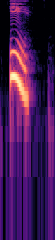
\includegraphics[width=\textwidth]{res/images/model/I.png}
        \caption{Vowel 'I' Spectrogram}
        \label{fig:vowel_i_spec}
    \end{subfigure}
    \hfill
    \begin{subfigure}[b]{0.19\textwidth}
        
\includegraphics[width=\textwidth]{res/images/model/O.png}
        \caption{Vowel 'O' Spectrogram}
        \label{fig:vowel_o_spec}
    \end{subfigure}
    \hfill
    \begin{subfigure}[b]{0.19\textwidth}
        
\includegraphics[width=\textwidth]{res/images/model/U.png}
        \caption{Vowel 'U' Spectrogram}
        \label{fig:vowel_u_spec}
    \end{subfigure}
    \caption{Example Spectrograms for Each Italian Vowel}
    \label{fig:vowel_spectrograms}
\end{figure}

\paragraph{}
Each spectrogram reveals distinct characteristics: vowel 'A' shows strong energy concentration in lower frequencies, 'E' exhibits clear formant structure in mid-range frequencies, 'I' displays high-frequency energy distribution, while 'O' and 'U' demonstrate characteristic low-frequency patterns. These visual representations serve as the input for our CNN model, providing a standardized format for vowel classification.

\subsection{Image Specifications}

\paragraph{}
The spectrogram images are generated with specific technical specifications to ensure optimal quality and consistency across the dataset. Each image is produced with dimensions of 240x55 pixels, providing sufficient resolution to capture relevant spectral features while maintaining computational efficiency. The images are generated in grayscale format and visualized using the 'magma' colormap, which effectively represents the intensity variations in the spectrogram. All images are saved in PNG format, with careful attention to removing axes and margins to focus solely on the spectral content.

\subsection{Processing Pipeline}

\paragraph{}
The processing pipeline consists of three main stages: audio loading, spectrogram computation, and image generation. The audio loading stage utilizes librosa's load function with the following implementation:

\begin{lstlisting}[language=Python, caption={Audio Loading Code}]
y, sr = librosa.load(audio_path, sr=None)
\end{lstlisting}

\paragraph{}
The spectrogram computation stage implements mel-spectrogram generation with carefully tuned parameters:

\begin{lstlisting}[language=Python, caption={Spectrogram Generation Code}]
mel_spect = librosa.feature.melspectrogram(
    y=y,
    sr=sr,
    n_fft=2048,
    hop_length=512,
    n_mels=128,
    fmin=20,
    fmax=8000
)
mel_spect_db = librosa.power_to_db(mel_spect, ref=np.max)
\end{lstlisting}

\paragraph{}
The final image generation stage involves creating figures with specific dimensions, plotting spectrograms using librosa's display function, removing axes and margins for clarity, and saving the results as high-quality PNG files. This process ensures consistent and high-quality visual representations of the vowel sounds.

\subsection{File Organization}
\label{subsec:image-organization}

\paragraph{}
The image dataset follows a structured organization system designed for efficient access and processing. Images are systematically organized in class-specific directories (A, E, I, O, U), with a consistent naming convention following the pattern \texttt{[vowel]\_[index].png}. Each image represents the spectral content of a specific vowel sound, maintaining a direct correspondence with its source audio file.

\paragraph{}
The naming convention ensures:
\begin{itemize}
    \item Easy identification of vowel class
    \item Direct mapping to source audio files
    \item Sequential organization within each class
    \item Consistent file format across the dataset
\end{itemize}

\section{CNN Model Implementation}
\label{sec:cnn-implementation}

\paragraph{}
After preparing the spectrogram images, we implemented a Convolutional Neural Network specifically designed for vowel recognition. The model architecture was optimized for processing the 240x55 pixel spectrograms while maintaining computational efficiency and high accuracy.

\subsection{Model Architecture}
\label{subsec:model-architecture}

\paragraph{}
The CNN model follows a sequential architecture with three main convolutional blocks followed by a classification head. Each convolutional block consists of a convolutional layer, batch normalization, and max pooling, progressively extracting higher-level features from the input spectrograms. The model architecture is implemented as follows:


\begin{algorithm}[ht]
    \caption{CNN Model}\label{alg:cnnmodel}
    \begin{algorithmic}
        \STATE \textbf{Define} build\_model()
        \STATE model $\gets$ Sequential([

        \STATE \quad \textit{\# Input layer: Accepts images with a single channel (grayscale)}
        \STATE \quad Input(shape=(IMG\_SIZE[0], IMG\_SIZE[1], 1)),  

        \STATE

        \STATE \quad \textit{\# First convolutional block}
        \STATE \quad Conv2D(32, 3, padding='same', activation='relu'),
        \STATE \quad BatchNormalization(),
        \STATE \quad MaxPooling2D(),

        \STATE

        \STATE \quad \textit{\# Second convolutional block}
        \STATE \quad Conv2D(64, 3, padding='same', activation='relu'),
        \STATE \quad BatchNormalization(),
        \STATE \quad MaxPooling2D(),
        
        \STATE

        \STATE \quad \textit{\# Third convolutional block}
        \STATE \quad Conv2D(128, 3, padding='same', activation='relu'),
        \STATE \quad BatchNormalization(),
        \STATE \quad MaxPooling2D(),

        \STATE

        \STATE \quad \textit{\# Fully connected layers for classification}
        \STATE \quad GlobalAveragePooling2D(),
        \STATE \quad Dropout(0.3),
        \STATE \quad Dense(64, activation='relu'),
        \STATE \quad BatchNormalization(),
        \STATE \quad Dense(NUM\_CLASSES, activation='softmax')

        \STATE ])
        
        \STATE

        \STATE \textbf{return} model
    \end{algorithmic}
\end{algorithm}



\subsection{Training Configuration}
\label{subsec:training-configuration}

\paragraph{}
The training process is configured with careful attention to optimization and regularization. We utilize the Adam optimizer with a learning rate of 1e-4, which provides good convergence while avoiding overshooting. The categorical cross-entropy loss function is employed for multi-class classification. The model is trained with a batch size of 8 and for up to 100 epochs, with early stopping to prevent overfitting.

\paragraph{}
Several callbacks are implemented to enhance the training process:

\begin{lstlisting}[language=Python, caption={Training Callbacks Configuration}]
callbacks = [
    tf.keras.callbacks.EarlyStopping(
        monitor='val_accuracy',
        patience=20,
        restore_best_weights=True
    ),
    tf.keras.callbacks.ReduceLROnPlateau(
        monitor='val_accuracy',
        factor=0.2,
        patience=5,
        min_lr=1e-6
    ),
    tf.keras.callbacks.ModelCheckpoint(
        'best_model.h5',
        save_best_only=True,
        monitor='val_accuracy'
    )
]
\end{lstlisting}

\subsection{Data Augmentation}
\label{subsec:data-augmentation}

\paragraph{}
To improve model robustness and prevent overfitting, we implement data augmentation during training. The augmentation pipeline includes subtle rotations, width and height shifts, and zoom variations, all carefully calibrated to maintain the spectral characteristics of the vowels while introducing meaningful variations to the training data.

\begin{lstlisting}[language=Python, caption={Data Augmentation Configuration}]
train_datagen = ImageDataGenerator(
    preprocessing_function=preprocess_image,
    rotation_range=5,
    width_shift_range=0.05,
    height_shift_range=0.05,
    zoom_range=0.05,
    fill_mode='constant',
    cval=0
)
\end{lstlisting}

\subsection{Model Evaluation}
\label{subsec:model-evaluation}

\paragraph{}
The model's performance is evaluated through comprehensive metrics including accuracy, loss curves, confusion matrices, and per-class performance analysis. We implement detailed visualization functions to track the training progress and analyze the model's behavior:

\begin{lstlisting}[language=Python, caption={Evaluation Visualization Code}]
def plot_training_history(history):
    fig, (ax1, ax2) = plt.subplots(1, 2, figsize=(15, 5))
    
    # Accuracy plot
    ax1.plot(history.history['accuracy'], label='Training')
    ax1.plot(history.history['val_accuracy'], label='Validation')
    ax1.set_title('Model Accuracy')
    ax1.set_xlabel('Epoch')
    ax1.set_ylabel('Accuracy')
    ax1.legend()
    
    # Loss plot
    ax2.plot(history.history['loss'], label='Training')
    ax2.plot(history.history['val_loss'], label='Validation')
    ax2.set_title('Model Loss')
    ax2.set_xlabel('Epoch')
    ax2.set_ylabel('Loss')
    ax2.legend()
\end{lstlisting}

\paragraph{}
The evaluation results are systematically documented, including detailed performance metrics for each vowel class, confusion matrices to analyze misclassification patterns, and confidence distribution analysis to assess the model's prediction reliability. This comprehensive evaluation approach ensures thorough understanding of the model's strengths and limitations in vowel recognition tasks.


\paragraph{}
This chapter has presented a comprehensive description of our vowel recognition system's implementation, encompassing three main components: audio data generation, spectrogram conversion, and CNN model architecture. The audio generation pipeline creates a diverse dataset of Italian vowel sounds using multiple TTS engines, ensuring broad coverage of pronunciation variations. The spectrogram generation system transforms these audio samples into standardized visual representations, carefully preserving the acoustic features crucial for vowel identification. The CNN model implementation leverages modern deep learning techniques, including batch normalization, dropout regularization, and data augmentation, to achieve robust vowel classification.

\paragraph{}
The systematic approach to data preparation and model design establishes a solid foundation for accurate vowel recognition. Each component has been carefully optimized and integrated, from the initial audio synthesis to the final neural network architecture. The detailed training configuration and evaluation framework provide a comprehensive structure for model assessment. The extensive experimental results, including detailed performance metrics, confusion matrices, and per-class analyses, will be thoroughly discussed in Chapter 6, where we present a comprehensive evaluation of the system's performance across various testing scenarios.

